
\documentclass[10pt,twoside]{article}
\usepackage{ComplexSystems}
\usepackage[T1]{fontenc}
\usepackage[utf8]{inputenc}
\usepackage{amsmath,amssymb}
\usepackage{graphicx,booktabs,microtype,url}
\usepackage[hidelinks]{hyperref}
\usepackage[numbers,sort&compress]{natbib}
\graphicspath{{figures/}}


\DeclareMathOperator*{\argmin}{arg\,min}
\newcommand{\bs}{\mathbf{s}}
\newcommand{\bD}{\mathbf{D}}
\newcommand{\bx}{\mathbf{x}}
\newcommand{\NML}{\operatorname{NML}}
\newcommand{\NLL}{\operatorname{NLL}}
\newcommand{\Hb}{H_b}
\newcommand{\orbit}{\mathcal{O}}

\copyrightinfo{Draft}{2026}{1}{1+}
\markboth{Relative-Periodic Domain Selection}{Selecting periodic domains in CA spacetime with Bernoulli NML}
\pagestyle{nofooters}

\title{Selecting Periodic Domains in Cellular Automaton Spacetime with Bernoulli NML}

\author{Author One\\
Department of X, Institution Y\\
City, Country\\
\texttt{author1@example.com}\\[6pt]
\and
Author Two\\
Department of X, Institution Y\\
City, Country}

\begin{document}
\maketitle

\noindent Cellular automata often generate spacetime patterns with large regular domains punctuated by defects and particle-like activity. A fast way to detect the dominant periodic organization of those domains is introduced by combining relative-periodic orbit partitions with a Bernoulli normalized maximum likelihood score. The method projects each candidate period/shift pair to its nearest periodic background by orbit-wise majority vote, then balances fit against complexity. A structural theorem identifies exactly when larger templates universally refine smaller ones, explaining why raw defect minimization and Bernoulli likelihood overfit. A second theorem specializes classical MDL/NML rate separation to show eventual exclusion of asymptotically inferior candidates and stabilization when the best rate is unique. Experiments in one, two, and three dimensions support the theory and show that the complexity penalty is essential for avoiding period inflation.


\section{Introduction}

Cellular automata (CA) frequently produce spacetime patterns in which large regular domains coexist with defects, particles, and interfaces. For complex-systems analysis, these domains matter because they are often the stage on which information transmission, coherent structures, and emergent computation become visible. A natural question is therefore: given a finite CA spacetime, what is the simplest global periodic organization that best explains it, and what residual structure remains after that organization is removed?

Two established traditions address nearby problems. Computational mechanics and local causal-state methods reconstruct local statistical structure and can identify domains, particles, and interactions in rich detail \cite{crutchfield1997,hanson1992,rupe2018,shalizi2006}. Compression-based and survey-based work classifies rules globally and at scale \cite{packard1985,boccara1999,zenil2010}. These approaches optimize different objectives. Local models provide rich dynamical semantics, while broad surveys remain computationally light. The present paper aims at a middle ground: a global, fast, complexity-penalized selector for periodic spacetime templates that can be used across many rules while still supporting theorem-level analysis.

The method is based on \emph{relative-periodic orbit classes}. For a candidate period and shift, the corresponding spacetime translation partitions the observed field into orbit classes. The nearest binary background satisfying that symmetry is obtained by a majority vote on each orbit class. Candidates are then scored by a Bernoulli normalized maximum likelihood (NML) criterion defined over those orbit classes. The procedure is therefore top-down: fit the best global periodic background, then study the residual mask for particle-rich or otherwise structured departures.

This contribution should be positioned carefully. The paper does not claim that periodic domains, defects, or particles are new objects in CA research. Rather, it introduces a tractable global selector for periodic domains, together with a model-family-specific analysis of when larger templates necessarily overfit, when NML selection stabilizes, and when background period is or is not identifiable. The emphasis is on a coherent package: a model family, a selector, a structural theorem explaining overcapacity, a stabilization theorem for this family, and empirical evidence that the package is useful on CA spacetimes.

\begin{figure}[t]
\centering
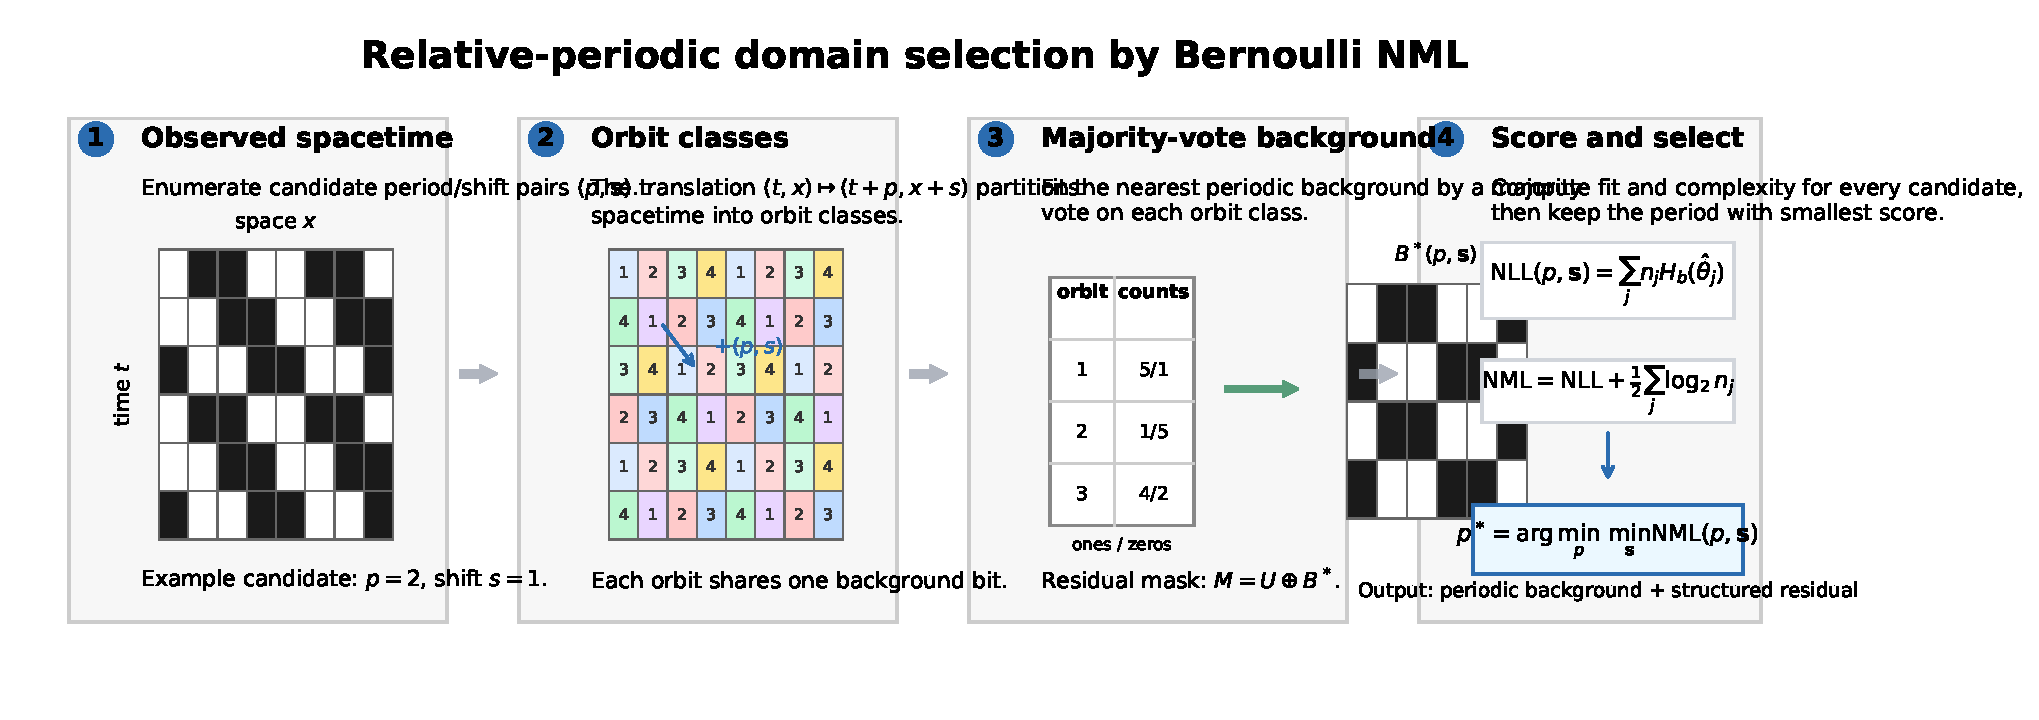
\includegraphics[width=0.99\linewidth]{algorithm_detailed.pdf}
\caption{Relative-periodic domain selection by Bernoulli NML. The first sentence of the caption serves as a title. Starting from an observed spacetime, the method enumerates candidate period/shift pairs, induces an orbit partition for each candidate, constructs the nearest majority-vote background, and scores the candidate by a Bernoulli NML criterion. The output is a selected periodic background together with a residual mask that isolates structured departures from that background.}
\label{fig:algorithm}
\end{figure}

\section{Relative-periodic orbit classes}

\begin{definition}
Given a binary spacetime $U \in \{0,1\}^{T \times D_1 \times \cdots \times D_n}$, shift $\bs \in \mathbb{Z}^n$, and period $p \geq 1$, the relative-periodic model class $\mathcal{B}(p,\bs)$ consists of all fields $B$ satisfying
\[
B[t+p,\,\bx+\bs \bmod \bD] = B[t,\bx]
\]
for all valid indices. The corresponding spacetime translation partitions the observation into orbit classes $\{O_j\}_{j=1}^{k}$ where $k = p\prod_i D_i$. A candidate background assigns one binary value to each orbit class.
\end{definition}

The basic computational advantage is immediate. A global spacetime template is represented by a finite partition, and fitting that template becomes a set of local decisions on partition elements.

\begin{lemma}
Let $n_j^{(1)}$ and $n_j^{(0)}$ be the number of ones and zeros observed in orbit class $O_j$. The Hamming distance from $U$ to $\mathcal{B}(p,\bs)$ is minimized by assigning to each orbit class its majority symbol. The minimum residual count is $\sum_j \min\{n_j^{(0)},n_j^{(1)}\}$.
\end{lemma}

\begin{proof}
The Hamming distance decomposes additively over orbit classes. Because a candidate background is constant on each orbit class, the optimal bit in that class is simply the majority value.
\end{proof}

This orbit-class reduction is classical in spirit, but in the present setting it is the key mechanism that turns spacetime fitting into a tractable model-selection problem.

\section{Structural divisibility and the NML selector}

The main structural issue is overcapacity. Larger templates often fit better simply because they have more orbit classes. The first theorem identifies exactly when that improvement is guaranteed.

\begin{theorem}\label{thm:div}
Let $c_1=(p_1,\bs_1)$ and $c_2=(p_2,\bs_2)$ be relative-periodic candidates. The following are equivalent:
\begin{enumerate}
\item[(i)] $p_2 = m p_1$ and $\bs_2 \equiv m\bs_1 \pmod{\bD}$ for some integer $m\ge 1$.
\item[(ii)] The orbit partition induced by $c_2$ refines the orbit partition induced by $c_1$.
\item[(iii)] $\mathcal{B}(p_1,\bs_1) \subseteq \mathcal{B}(p_2,\bs_2)$.
\item[(iv)] For every binary spacetime $U$, the optimal Hamming residual satisfies $d_U^*(c_2) \le d_U^*(c_1)$.
\item[(v)] For every binary spacetime $U$, the Bernoulli negative log-likelihood satisfies $\NLL_U(c_2) \le \NLL_U(c_1)$.
\end{enumerate}
Hence along constant-velocity divisibility chains, both residual count and Bernoulli NLL are monotone non-increasing.
\end{theorem}

\begin{proof}
Condition (i) states that the spacetime translation for $c_2$ is a power of the translation for $c_1$, which is equivalent to refinement of orbit partitions. Refinement implies model nesting, and model nesting implies that optimization over the larger class cannot worsen the optimum Hamming residual. Refinement also implies the NLL inequality because splitting an orbit class can only decrease Bernoulli NLL by concavity of binary entropy. For necessity, suppose refinement fails. Then some orbit of $c_2$ intersects two distinct orbits of $c_1$. Construct a spacetime that is constant on each $c_1$ orbit but takes different values on those two classes. Candidate $c_1$ achieves zero residual and zero NLL, while $c_2$ necessarily mixes symbols in one orbit and therefore incurs positive residual and positive NLL. Thus the universal inequalities hold only under refinement.
\end{proof}

Theorem~\ref{thm:div} explains why raw defect minimization and Bernoulli likelihood overfit. Along velocity-matched divisibility chains, larger templates are guaranteed to fit at least as well. A complexity penalty is therefore indispensable.

For a candidate $(p,\bs)$ with orbit classes $O_j$, let $n_j = |O_j|$ and $\hat\theta_j = n_j^{(1)}/n_j$. Define
\[
\NML(p,\bs) = \sum_j n_j\,\Hb(\hat\theta_j) + \frac{1}{2}\sum_j \log_2 n_j,
\]
where $\Hb(\theta)$ is the binary entropy. The first term is the Bernoulli negative log-likelihood, and the second is the asymptotic NML complexity for independent Bernoulli classes \cite{grunwald2007,shtarkov1987}. The selected candidate minimizes this score over the scanned period/shift family.

\section{Stabilization and identifiability}

The next theorem is a specialization of standard MDL/NML rate-separation logic to relative-periodic orbit-class models.

\begin{theorem}\label{thm:stab}
Let $\mathcal{C}$ be a fixed finite candidate set. Assume that, for each candidate $c$ and each orbit class $j$, the empirical frequency $\hat\theta_j(T)$ converges to a limit $\theta_j^*$. Define the per-site NLL rate
\[
\lambda_c = \frac{1}{k_c}\sum_j \Hb(\theta_j^*).
\]
Then
\[
\NML(c,T)=\lambda_c N(T)+\frac{k_c}{2}\log_2 T + o(N(T)).
\]
Every candidate with $\lambda_c$ strictly above the minimum is eventually excluded, and if the minimum rate is unique then the NML selector stabilizes to a single winner.
\end{theorem}

\begin{proof}
Convergent orbit-class frequencies imply convergence of the Bernoulli NLL rate by continuity of binary entropy and the fact that each orbit class contains $T/p_c+O(1)$ observations. The complexity term contributes $\frac{k_c}{2}\log_2 T+O(1)$. If two candidates have distinct rates, the linear fit gap dominates the logarithmic complexity gap for sufficiently large $T$. Finite candidate sets then give eventual exclusion of every non-minimizer, and uniqueness of the minimum rate gives locking.
\end{proof}

The theorem proves eventual ordering between candidates with distinct asymptotic rates; it does not by itself resolve exact ties at the rate level.

A complementary construction shows that background period is not identifiable in general.

\begin{theorem}\label{thm:nonid}
For any candidate $(p_0,\bs)$, there exist spacetimes for which a larger velocity-matched multiple eventually beats $(p_0,\bs)$ under Bernoulli NML.
\end{theorem}

\begin{proof}[Proof sketch]
Construct a spacetime whose residual under $(p_0,\bs)$ is itself periodic with period multiplier $q>1$. The larger candidate $(qp_0,q\bs)$ absorbs that residual periodicity and attains zero asymptotic Bernoulli rate, while $(p_0,\bs)$ retains a positive rate. Theorem~\ref{thm:stab} then implies eventual dominance of the larger template.
\end{proof}

On the positive side, if the spacetime becomes exactly relative-periodic after a finite transient, then the smallest period is recovered because all larger velocity-matched multiples share the same zero asymptotic rate but pay a larger logarithmic complexity penalty.

\section{Experiments}

The empirical program has three purposes. First, it tests the stabilization prediction in one, two, and three dimensions. Second, it isolates the role of the complexity penalty by comparing the NML selector with raw residual minimization and Bernoulli NLL. Third, it asks whether the residual masks reveal interesting structured defects once a global domain has been selected.

\subsection{Cross-dimensional stabilization}

In one dimension, the selector was applied to elementary cellular automata rules 30, 54, and 110 on a ring of width $192$ with candidate periods $1$ through $10$ and shifts from $-6$ to $+6$. In two dimensions, the study included broad Life-like and totalistic surveys on periodic grids together with detailed horizon sweeps for representative persistent-residual rules. In three dimensions, a totalistic ``diamoeba3d'' rule was scanned on a $16^3$ torus.

Figure~\ref{fig:stabilization} shows representative stabilization patterns. Rule 54 locks immediately to period $4$ with steadily increasing margin. Rule 110 exhibits a short transient before settling at period $4$ under the period-first search. S24/B11 in two dimensions displays the characteristic pre-transition margin dip expected when the selector is approaching a period change. The three-dimensional rule stabilizes to period $1$ from the first measured horizon, again with steadily growing margin.

\begin{figure*}[t]
\centering

\includegraphics[width=0.97\textwidth]{stabilization_summary.png}
\caption{Representative stabilization patterns across one-, two-, and three-dimensional rules. The top row shows selected period versus horizon; the bottom row shows the NML margin to the runner-up candidate. After the final transition, margins grow rather than shrink. This is the empirical signature expected when the asymptotic rate gap dominates the logarithmic complexity penalty.}
\label{fig:stabilization}
\end{figure*}

Across the nine detailed case studies reported in the source manuscript, every rule made at most two period transitions before the selected period locked over the observed horizon range. That pattern does not prove asymptotic stabilization, but it is exactly what Theorem~\ref{thm:stab} predicts when the rate-minimizer is unique.

\subsection{Selector ablation}

The selector comparison is especially revealing. When the same candidate family is scored by raw residual count, by Bernoulli NLL, and by Bernoulli NML, only the NML score avoids systematic period inflation. Figure~\ref{fig:ablation} summarizes the Life-like survey at $T=100$. Bernoulli NLL selects the highest available period for every nontrivial rule in the survey. Residual minimization also favors high periods. Bernoulli NML instead concentrates mass at period $1$, with only a small minority of rules supporting periods $2$ or greater. This is the empirical manifestation of Theorem~\ref{thm:div}: once refinement guarantees monotone fit improvement, only complexity regularization can prevent overfitting.

\begin{figure}[t]
\centering
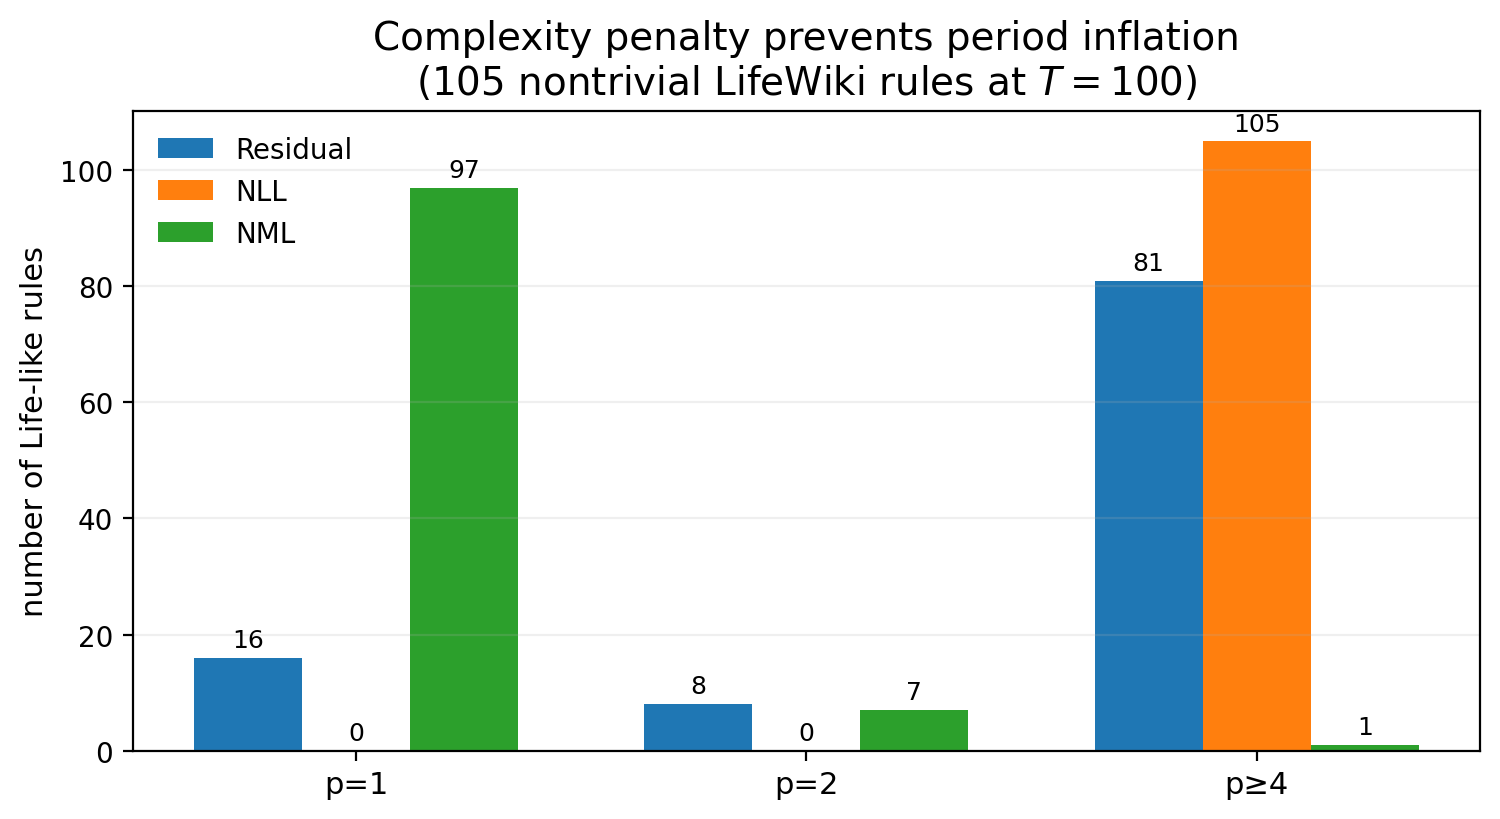
\includegraphics[width=0.98\linewidth]{selector_ablation.png}
\caption{Selector comparison on 105 nontrivial Life-like rules at $T=100$. Raw residual minimization and Bernoulli NLL are pulled toward larger periods because fit can only improve along divisibility chains. The Bernoulli NML penalty prevents that period inflation and yields parsimonious selections.}
\label{fig:ablation}
\end{figure}

\subsection{Residual structure}

The selected background is useful not only because it identifies a domain hypothesis, but also because the residual mask preserves structured departures from that hypothesis. For rules such as S37/B11, the residual density remains approximately constant as the grid size increases, indicating an extensive bulk defect phenomenon rather than a small finite-size artifact. In one dimension, an entropy-rate comparison also shows that the periodic background captures the predictable part of the spacetime while the residual retains substantial but structured uncertainty.

\begin{figure*}[t]
\centering
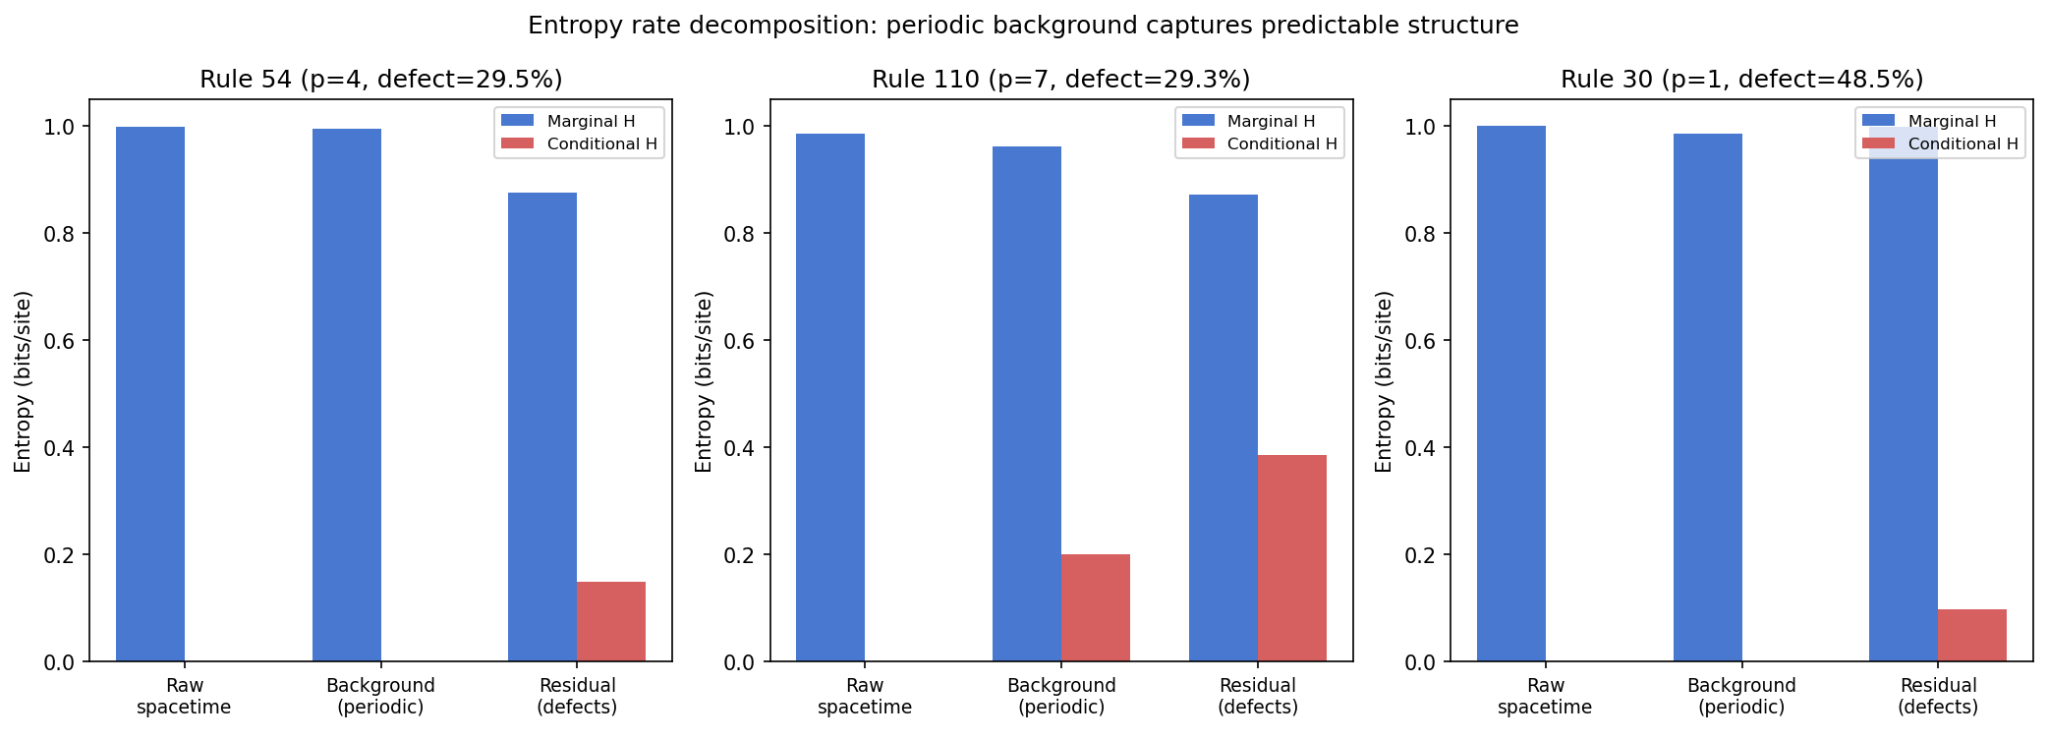
\includegraphics[width=0.97\textwidth]{entropy_rate_comparison.png}
\caption{Entropy-rate decomposition for rules 54, 110, and 30. The raw spacetime is deterministic given a sufficient local context. The periodic background retains nearly all of that predictability, while the residual mask has much lower conditional entropy than marginal entropy. This indicates that the residual is not just random noise; it retains internal spatiotemporal structure consistent with particle-like dynamics.}
\label{fig:entropy}
\end{figure*}

\section{Discussion}

The main methodological point is that periodic-domain selection can be formulated as an ordinary model-selection problem once CA spacetime is represented through orbit partitions. That representation makes three things possible. First, fitting is fast because it reduces to majority voting on orbit classes. Second, the overcapacity of larger templates becomes explicit through partition refinement. Third, stabilization can be analyzed with standard MDL/NML asymptotics once orbit-class frequencies converge.

The framework also has clear limits. It selects the best-compressing global period, not necessarily a physicist's ``true'' background period. The nonidentifiability theorem shows that structured residual periodicity can force a larger template to win. The Bernoulli orbit model also treats observations within an orbit class as independent, which is an asymptotic convenience rather than a literal generative description.

From a complex-systems viewpoint, the method is best understood as a scalable front end for structure discovery. It does not replace causal-state or particle analysis, but it does provide a fast global domain hypothesis and a residual mask that shows where more detailed local analysis is likely to pay off.

\section{Conclusion}

Bernoulli NML provides a simple global way to select periodic domains in cellular automaton spacetime. Within a fixed candidate family, asymptotically inferior templates are eventually excluded, and when the best rate is unique the selected period stabilizes. The experiments support this picture in one, two, and three dimensions, while also showing that the complexity penalty is essential for avoiding systematic period inflation.

The broader contribution is a compact bridge between information-theoretic model selection and the study of emergent spacetime organization. A selected periodic background serves as a domain hypothesis; the residual mask isolates the structured departures from that hypothesis that are most relevant for particles, defects, and coherent-structure analysis.

\begin{thebibliography}{10}

\bibitem{boccara1999}
N. Boccara and M. Roger, ``Totalistic Two-Dimensional Cellular Automata Exhibiting Global Periodic Behavior,'' \emph{International Journal of Modern Physics C}, 10(6), 1051--1066 (1999).

\bibitem{crutchfield1997}
J. P. Crutchfield and J. E. Hanson, ``Computational Mechanics of Cellular Automata: An Example,'' \emph{Physica D}, 103, 169--189 (1997).

\bibitem{grunwald2007}
P. Gr{"u}nwald, \emph{The Minimum Description Length Principle}. MIT Press, Cambridge, MA (2007).

\bibitem{hanson1992}
J. E. Hanson and J. P. Crutchfield, ``The Attractor-Basin Portrait of a Cellular Automaton,'' \emph{Journal of Statistical Physics}, 66, 1415--1462 (1992).

\bibitem{packard1985}
N. H. Packard and S. Wolfram, ``Two-Dimensional Cellular Automata,'' \emph{Journal of Statistical Physics}, 38, 901--946 (1985).

\bibitem{redeker2017}
M. Redeker, ``A Language for Particle Interactions in Rule 54 and Other Cellular Automata,'' \emph{Complex Systems}, 26(1), 1--32 (2017).

\bibitem{rupe2018}
A. Rupe and J. P. Crutchfield, ``Local Causal States and Discrete Coherent Structures,'' \emph{Chaos}, 28, 075312 (2018).

\bibitem{shalizi2006}
C. R. Shalizi, R. Haslinger, J.-B. Rouquier, K. L. Klinkner, and C. Moore, ``Automatic Filters for the Detection of Coherent Structure in Spatiotemporal Systems,'' \emph{Physical Review E}, 73, 036104 (2006).

\bibitem{shtarkov1987}
Y. M. Shtarkov, ``Universal Sequential Coding of Single Messages,'' \emph{Problems of Information Transmission}, 23, 3--17 (1987).

\bibitem{zenil2010}
H. Zenil, ``Compression-Based Investigation of the Dynamical Properties of Cellular Automata and Other Systems,'' \emph{Complex Systems}, 19(1), 1--28 (2010).

\end{thebibliography}

\end{document}